\documentclass[journal,12pt,twocolumn]{IEEEtran}

\usepackage{setspace}
\usepackage{gensymb}
\singlespacing
\usepackage[cmex10]{amsmath}
\usepackage{cancel}
\usepackage{amsthm}
\usepackage{amsmath}
\usepackage{paralist}
\usepackage{upgreek}
\usepackage{mathrsfs}
\usepackage{txfonts}
\usepackage{stfloats}
\usepackage{bm}
\usepackage{cite}
\usepackage{cases}
\usepackage{subfig}

\usepackage{longtable}
\usepackage{multirow}
\usepackage{enumitem}
\usepackage{mathtools}
\usepackage{steinmetz}
\usepackage{tikz}
\usepackage{circuitikz}
\usepackage{verbatim}
\usepackage{tfrupee}
\usepackage[breaklinks=true]{hyperref}
\usepackage{graphicx}
\usepackage{tkz-euclide}

\usetikzlibrary{calc,math}
\usepackage{listings}
    \usepackage{color}                                            %%
    \usepackage{array}                                            %%
    \usepackage{longtable}                                        %%
    \usepackage{calc}                                             %%
    \usepackage{multirow}                                         %%
    \usepackage{hhline}                                           %%
    \usepackage{ifthen}                                           %%
    \usepackage{lscape}     
\usepackage{multicol}
\usepackage{chngcntr}

\DeclareMathOperator*{\Res}{Res}
\usepackage{romannum}
\renewcommand\thesection{\arabic{section}}
\renewcommand\thesubsection{\thesection.\arabic{subsection}}
\renewcommand\thesubsubsection{\thesubsection.\arabic{subsubsection}}

\renewcommand\thesectiondis{\arabic{section}}
\renewcommand\thesubsectiondis{\thesectiondis.\arabic{subsection}}
\renewcommand\thesubsubsectiondis{\thesubsectiondis.\arabic{sub subsection}}


\hyphenation{optical networks semiconduc-tor}
\def\inputGnumericTable{}                                 %%

\lstset{
%language=C,
frame=single, 
breaklines=true,
columns=fullflexible
}
\date{March 2021}

\begin{document}

\newcommand{\multlinecomment}[1]{\directlua{-- #1}}
\newcommand{\BEQA}{\begin{eqnarray}}
\newcommand{\EEQA}{\end{eqnarray}}
\newcommand{\define}{\stackrel{\triangle}{=}}
\bibliographystyle{IEEEtran}
\raggedbottom
\setlength{\parindent}{0pt}
\providecommand{\mbf}{\mathbf}
\providecommand{\pr}[1]{\ensuremath{\Pr\left(#1\right)}}
\providecommand{\qfunc}[1]{\ensuremath{Q\left(#1\right)}}
\providecommand{\fn}[1]{\ensuremath{f\left(#1\right)}}
\providecommand{\e}[1]{\ensuremath{E\left(#1\right)}}
\providecommand{\sbrak}[1]{\ensuremath{{}\left[#1\right]}}
\providecommand{\lsbrak}[1]{\ensuremath{{}\left[#1\right.}}
\providecommand{\rsbrak}[1]{\ensuremath{{}\left.#1\right]}}
\providecommand{\brak}[1]{\ensuremath{\left(#1\right)}}
\providecommand{\lbrak}[1]{\ensuremath{\left(#1\right.}}
\providecommand{\rbrak}[1]{\ensuremath{\left.#1\right)}}
\providecommand{\cbrak}[1]{\ensuremath{\left\{#1\right\}}}
\providecommand{\lcbrak}[1]{\ensuremath{\left\{#1\right.}}
\providecommand{\rcbrak}[1]{\ensuremath{\left.#1\right\}}}
\theoremstyle{remark}
\newtheorem{rem}{Remark}
\newcommand{\sgn}{\mathop{\mathrm{sgn}}}
\providecommand{\abs}[1]{\vert#1\vert}
\providecommand{\res}[1]{\Res\displaylimits_{#1}} 
\providecommand{\norm}[1]{\lVert#1\rVert}
%\providecommand{\norm}[1]{\lVert#1\rVert}
\providecommand{\mtx}[1]{\mathbf{#1}}
\providecommand{\mean}[1]{E[ #1 ]}
\providecommand{\fourier}{\overset{\mathcal{F}}{ \rightleftharpoons}}
%\providecommand{\hilbert}{\overset{\mathcal{H}}{ \rightleftharpoons}}
\providecommand{\system}{\overset{\mathcal{H}}{ \longleftrightarrow}}
	%\newcommand{\solution}[2]{\textbf{Solution:}{#1}}
\newcommand{\solution}{\noindent \textbf{Solution: }}
\newcommand{\cosec}{\,\text{cosec}\,}
\providecommand{\dec}[2]{\ensuremath{\overset{#1}{\underset{#2}{\gtrless}}}}
\newcommand{\myvec}[1]{\ensuremath{\begin{pmatrix}#1\end{pmatrix}}}
\newcommand{\mydet}[1]{\ensuremath{\begin{vmatrix}#1\end{vmatrix}}}
\numberwithin{equation}{subsection}
\makeatletter
\vspace{3cm}
\title{Quiz-2}
\author{Arun SIddardha - AI20BTECH11019}
\maketitle
\newpage
\bigskip
\renewcommand{\thetable}{\theenumi}

%
Download latex code from 
%
\begin{lstlisting}
https://github.com/ArunSiddardha/EE900/tree/main/Quiz2
\end{lstlisting}

\section{Question}
A casual LTI systemhas impulse response h[n],for which z-transform is:
\begin{align}
    H(z)&=\frac{1+z^{-1}}{(1-\frac{1}{2}z^{-1})(1+\frac{1}{4}z^{-1})}
\end{align}
\begin{enumerate}
    \item What is the region of covergence of H(z)?
    \item Is the system stable ? Explain
\end{enumerate}
\section{Solution}
a) The above equation can be written as 
\begin{align}
    H(z)&=\frac{1+z}{(z-\frac{1}{2})(z+\frac{1}{4})}\\
    &= \frac{2}{z-\frac{1}{2}}-\frac{1}{z+\frac{1}{4}}\\
    &= 4 \times\frac{\frac{1}{2}z^{-1}}{1-\frac{1}{2}z^{-1}} + 4\times\frac{-\frac{1}{4}z^{-1}}{1-(-\frac{1}{4})z^{-1}}
\end{align}
ROC for first part is $\mid z\mid \; > \; \mid \frac{1}{2} \mid$ . ROC for second part is  $\mid z \mid \;>\; \mid \frac{1}{4} \mid$. The intersection gives the ROC which is 
The poles of the z-transform are given by $\mid z\mid \; > \; \mid \frac{1}{2} \mid$
\begin{align}
    z=\frac{1}{2},-\frac{1}{4}
\end{align}
The zero of the z-transform is given by 
\begin{align}
    z=-1
\end{align}

\begin{figure}[htp]
    \centering
    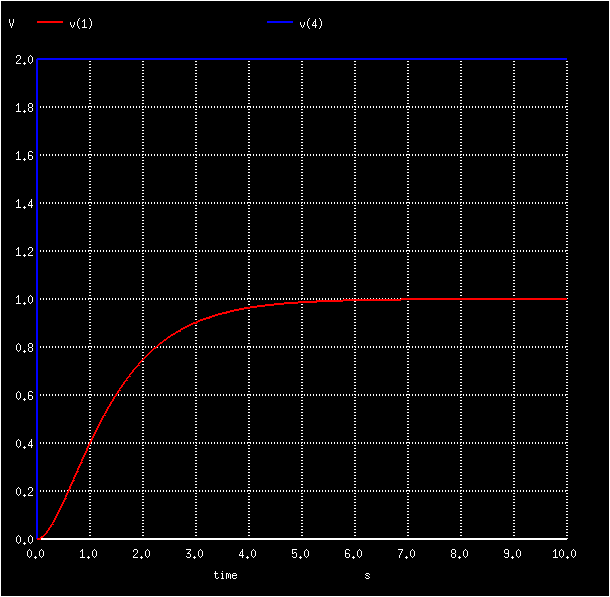
\includegraphics[width=\columnwidth]{fig.png}
    \caption{Pole-zero plot of the system}
    \label{fig:my_label}
\end{figure}
b)By defintition a causal system is stable if and only if all the poles of the Z-transform of the impulse response of the system lie inside the unit circle. So,since ROC include $\mid z \mid \; = 1$ the system is \textbf{stable}.

\end{document}

